\chapter{Обзор существующих решений}
\label{sec:Chapter2} \index{Chapter2}

Основным критерием поиска подходящего программного обеспечения является его возможность работать с уровнем синтеза  L1, то есть Single Look Complex (SLC). Ниже приведен список приложений для работы с SLC:\\

\section{Открытое программное обеспечения для работы с РЛИ уровня SLC}

1. SNAP - Платформа приложений Sentinel.\\
2. SARscape - это полный набор функций для комплексной обработки всех космических и отдельных авиационных радиолокационных данных.\\
3. GMTSAR - Система обработки InSAR в сочетании с GMT.\\
4. ISCE2 - Научная вычислительная среда InSAR.\\
5. Doris - Делфтское объектно-ориентированное радарно-интерферометрическое программное обеспечение.\\
6. SARPROZ - Инструмент для обработки SAR.\\
7. StaMPS/MTI - Стэнфордский метод для стойких рассеивателей.\\
8. kite - Подвыборка в виде дерева квадрантов, анализ ковариации данных для моделирования смещения поверхности. Удаление точек доступа (эмпирическое и по ДЖЕЙКОБСУ). Загрузка данных из различных центров обработки данных.\\
9. sarpy - Библиотека Python для простой обработки сложных данных SAR с использованием стандарта NGA SIC.\\
10. ROI\_PAC - Sentinel1.\\
11. pygmtsar - Скрипты на Python для обработки GMTSAR.\\
12. Xarray-Sentinel - Серверная часть X-массива для обработки спутниковых данных Copernicus Sentinel-1.\\
13. Sarsen - Алгоритмы и инструменты для геометрической и радиометрической коррекции данных SAR Sentinel-1 с учетом рельефа местности.\\
14. pyroSAR - Фреймворк на Python для крупномасштабной обработки спутниковых данных SAR.\\
15. S1\_NRB - Прототип процессора для радиолокационного устройства с нормализованным обратным рассеянием Sentinel-1.\\
16. ALUs - Различные процессоры, использующие графический процессор, самый быстрый для обеспечения когерентности Sentinel-1 и обратного рассеяния.\\

\subsection{SNAP}
	Главным достоинством SNAP является возможность работы с различными пакетами данных с разных спутников. Также присутствуют инструменты для работы с шумами, геопривязкой, поляризационными изображениями. Есть все функции для постобработки изображений.\\
	
	
\begin{figure}[ht]
    \centering
    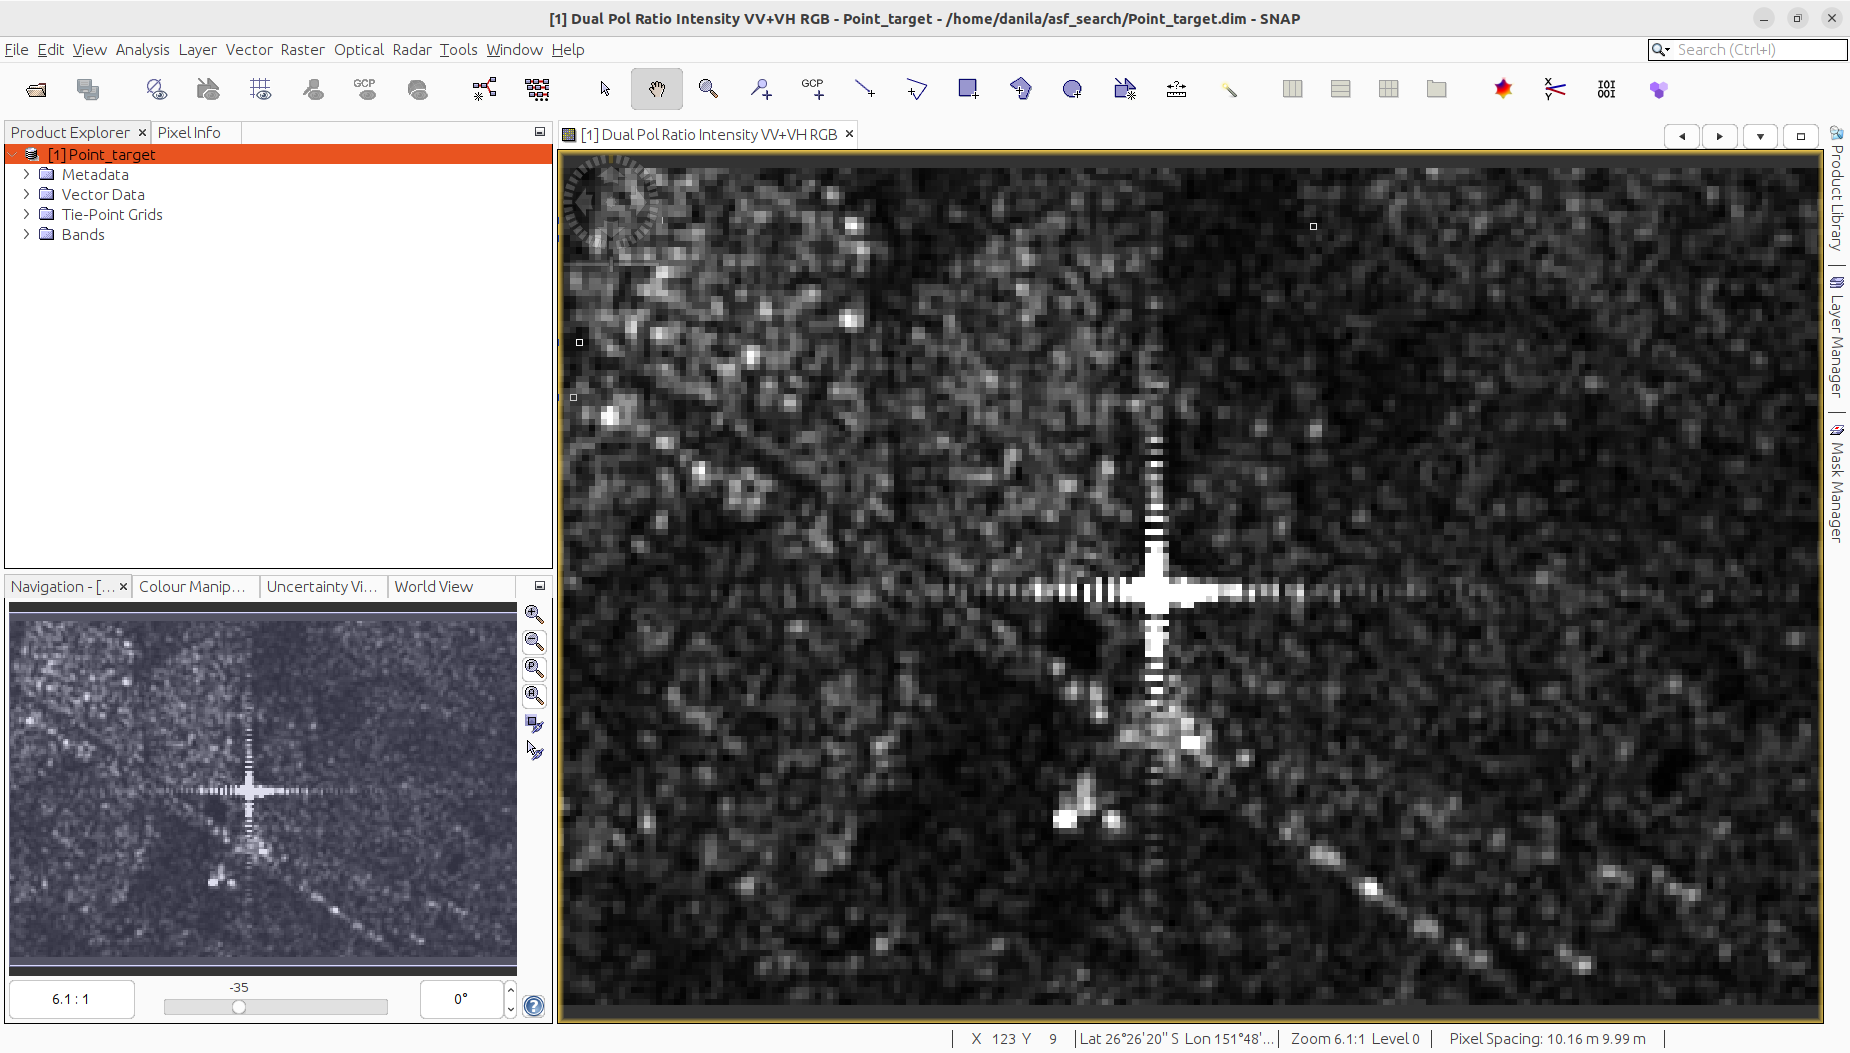
\includegraphics[width=0.8\textwidth]{snap.png}
    \caption{SNAP}
    \label{fig:snap}
\end{figure}

	
\subsection{SARscape}
	В данный момент приложение SARscape не доступно в России. Поэтому анализ невозможен.\\
	
\subsection{GMTSAR}		
	Данное программное обеспечение предоставляет возможности синтеза и постобработки изображений без графического интерфейса. Также присутсвуют функции для интерферометрической обработки.\\
	
\subsection{SARPROZ}
	Богатый функционал для работы с РЛИ уровня SLC.\\	

\begin{figure}[ht]
    \centering
    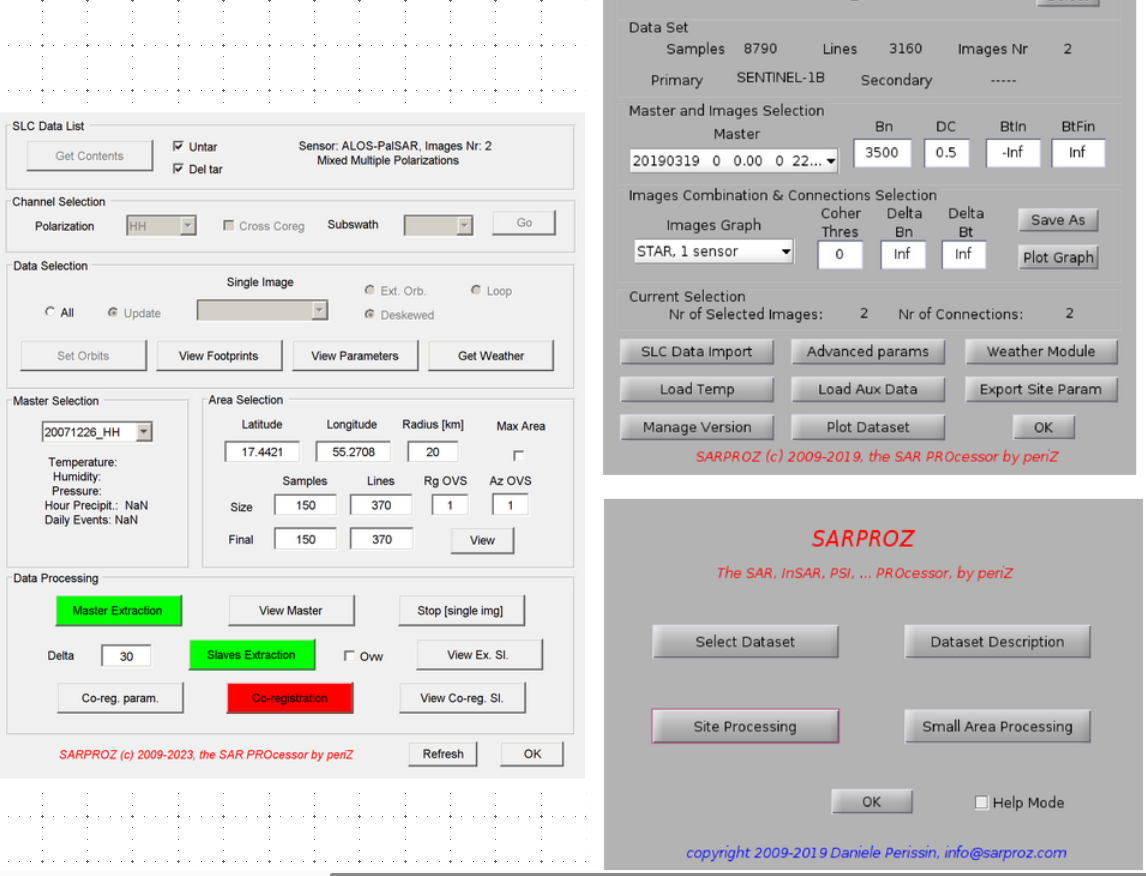
\includegraphics[width=0.8\textwidth]{sarproz.png}
    \caption{SARPROZ}
    \label{fig:sarproz}
\end{figure}
	
\subsection{StaMPS/MTI}

\section{Выводы}

	Все представленные выше программные комплексы не имеют возможности оценки разрешения РЛИ по точечным целям. Исключение составляет Radar Tools (RAT), но данное приложение написано на языке Interactive Data Language (IDL), лецензию на который невозможно получить из России. Также существует платформа SARvis, упомянутое в статье [], в котором также присутсвуют инструменты для определния разрешений РЛИ. Но найти данное приложение в открытом доступе не удалось
	
\newpage
